\documentclass[aspectratio=169]{beamer}
% talk-common.tex —— 各场分享共用的导言区配置
% 放在仓库根目录，由各个入口 .tex 通过 % talk-common.tex —— 各场分享共用的导言区配置
% 放在仓库根目录，由各个入口 .tex 通过 % talk-common.tex —— 各场分享共用的导言区配置
% 放在仓库根目录，由各个入口 .tex 通过 \input{talk-common.tex} 引用。
% 编译时需要把仓库根目录加入 TEXINPUTS，详见根目录 AGENTS.md 第 2 节。

\usetheme[customfont,showmaxslides,nofooterlogo]{pureminimalistic}
\usefonttheme{professionalfonts}
\usepackage[UTF8,fontset=none]{ctex}
\usepackage{graphicx}
\usepackage{listings}
\usepackage{appendixnumberbeamer}

\setsansfont{Fira Sans}
\setmonofont{Fira Mono}
\setCJKmainfont{Noto Sans CJK SC}
\setCJKsansfont{Noto Sans CJK SC}
\setCJKmonofont{Noto Sans CJK SC}

% 默认不引用上游示例 logo，有真实素材时再统一配置
\renewcommand{\logotitle}{}
\renewcommand{\logoheader}{}
\renewcommand{\logofooter}{}
\renewcommand{\pageword}{}

% 字号设置必须放在加载主题之后，避免被主题覆盖
\setbeamerfont{title}{size=\LARGE,shape=\upshape,series=\bfseries}
\setbeamerfont{presentation title}{shape=\upshape}
\setbeamerfont{frametitle}{size=\Large,shape=\upshape,series=\bfseries}

% 对浅色/深色都保持明确的代码对比度
\definecolor{TalkCodeBg}{HTML}{F3F4F6}
\definecolor{TalkCodeFg}{HTML}{17212B}
\definecolor{TalkCodeKeyword}{HTML}{174EA6}
\definecolor{TalkCodeComment}{HTML}{47634D}
\definecolor{TalkCodeString}{HTML}{8A3014}
\lstdefinestyle{talkcode}{
  basicstyle=\ttfamily\small\color{TalkCodeFg},
  backgroundcolor=\color{TalkCodeBg},
  keywordstyle=\bfseries\color{TalkCodeKeyword},
  commentstyle=\color{TalkCodeComment},
  stringstyle=\color{TalkCodeString},
  columns=fullflexible,
  keepspaces=true,
  showstringspaces=false,
  breaklines=true,
  tabsize=4,
  numbers=none,
  frame=none
}
\lstset{style=talkcode}
 引用。
% 编译时需要把仓库根目录加入 TEXINPUTS，详见根目录 AGENTS.md 第 2 节。

\usetheme[customfont,showmaxslides,nofooterlogo]{pureminimalistic}
\usefonttheme{professionalfonts}
\usepackage[UTF8,fontset=none]{ctex}
\usepackage{graphicx}
\usepackage{listings}
\usepackage{appendixnumberbeamer}

\setsansfont{Fira Sans}
\setmonofont{Fira Mono}
\setCJKmainfont{Noto Sans CJK SC}
\setCJKsansfont{Noto Sans CJK SC}
\setCJKmonofont{Noto Sans CJK SC}

% 默认不引用上游示例 logo，有真实素材时再统一配置
\renewcommand{\logotitle}{}
\renewcommand{\logoheader}{}
\renewcommand{\logofooter}{}
\renewcommand{\pageword}{}

% 字号设置必须放在加载主题之后，避免被主题覆盖
\setbeamerfont{title}{size=\LARGE,shape=\upshape,series=\bfseries}
\setbeamerfont{presentation title}{shape=\upshape}
\setbeamerfont{frametitle}{size=\Large,shape=\upshape,series=\bfseries}

% 对浅色/深色都保持明确的代码对比度
\definecolor{TalkCodeBg}{HTML}{F3F4F6}
\definecolor{TalkCodeFg}{HTML}{17212B}
\definecolor{TalkCodeKeyword}{HTML}{174EA6}
\definecolor{TalkCodeComment}{HTML}{47634D}
\definecolor{TalkCodeString}{HTML}{8A3014}
\lstdefinestyle{talkcode}{
  basicstyle=\ttfamily\small\color{TalkCodeFg},
  backgroundcolor=\color{TalkCodeBg},
  keywordstyle=\bfseries\color{TalkCodeKeyword},
  commentstyle=\color{TalkCodeComment},
  stringstyle=\color{TalkCodeString},
  columns=fullflexible,
  keepspaces=true,
  showstringspaces=false,
  breaklines=true,
  tabsize=4,
  numbers=none,
  frame=none
}
\lstset{style=talkcode}
 引用。
% 编译时需要把仓库根目录加入 TEXINPUTS，详见根目录 AGENTS.md 第 2 节。

\usetheme[customfont,showmaxslides,nofooterlogo]{pureminimalistic}
\usefonttheme{professionalfonts}
\usepackage[UTF8,fontset=none]{ctex}
\usepackage{graphicx}
\usepackage{listings}
\usepackage{appendixnumberbeamer}

\setsansfont{Fira Sans}
\setmonofont{Fira Mono}
\setCJKmainfont{Noto Sans CJK SC}
\setCJKsansfont{Noto Sans CJK SC}
\setCJKmonofont{Noto Sans CJK SC}

% 默认不引用上游示例 logo，有真实素材时再统一配置
\renewcommand{\logotitle}{}
\renewcommand{\logoheader}{}
\renewcommand{\logofooter}{}
\renewcommand{\pageword}{}

% 字号设置必须放在加载主题之后，避免被主题覆盖
\setbeamerfont{title}{size=\LARGE,shape=\upshape,series=\bfseries}
\setbeamerfont{presentation title}{shape=\upshape}
\setbeamerfont{frametitle}{size=\Large,shape=\upshape,series=\bfseries}

% 对浅色/深色都保持明确的代码对比度
\definecolor{TalkCodeBg}{HTML}{F3F4F6}
\definecolor{TalkCodeFg}{HTML}{17212B}
\definecolor{TalkCodeKeyword}{HTML}{174EA6}
\definecolor{TalkCodeComment}{HTML}{47634D}
\definecolor{TalkCodeString}{HTML}{8A3014}
\lstdefinestyle{talkcode}{
  basicstyle=\ttfamily\small\color{TalkCodeFg},
  backgroundcolor=\color{TalkCodeBg},
  keywordstyle=\bfseries\color{TalkCodeKeyword},
  commentstyle=\color{TalkCodeComment},
  stringstyle=\color{TalkCodeString},
  columns=fullflexible,
  keepspaces=true,
  showstringspaces=false,
  breaklines=true,
  tabsize=4,
  numbers=none,
  frame=none
}
\lstset{style=talkcode}


\usepackage[overridenote]{pdfpc}

\usepackage{tikz}
\usetikzlibrary{arrows.meta,calc,positioning}

\title[技术部第一次分享]{技术部第一次技术分享会}
\subtitle{技术部 2026 年活动总览}
\author{姚雨森}
\institute{技术部 分管主席}
\date{2026-10-16}

\begin{document}

\maketitle

\section{在技术部的一年，能收获什么}

\begin{frame}{在技术部的一年，能收获什么}
  这一年，技术部采取\textbf{技术分享会}与\textbf{小组协作开发}相结合的形式。
  \par\medskip
  \begin{vfilleditems}
    \item 学会几门编程语言，掌握常用的开发工具。
    \item 在真实项目中动手开发，获得实践经验。
    \item 对技术有自己的理解和品味。
    \item 认识新的同学，和大家一起交流、共同进步。
  \end{vfilleditems}
  \note{我们先讲讲，这一年在技术部，大家能收获什么。（读）}
\end{frame}

\section{这一年，技术部做什么}

\begin{frame}{这一年，技术部做什么}
  \begin{vfilleditems}
    \item \textbf{第一学期：软件开发的基本认识和实践}\par
      学习软件开发基础，通过重写一个简单项目积累实践经验。
    \item \textbf{寒假：开拓视野}\par
      学习其他编程语言和开发工具，了解软件开发的各个方向。
    \item \textbf{第二学期：真实项目实战}\par
      按照自身兴趣，参与协会真实生产项目的开发。
  \end{vfilleditems}
  \note{那为了这样的目标，我们就要有很多相应的活动，我们这一年的安排是这样的（读）}
\end{frame}

\section{第一学期的实践项目：ClinicAssistant}

\begin{frame}{ClinicAssistant：电脑诊所工具箱}
  \begin{itemize}
    \item 查看电脑的软硬件信息和运行状态。
    \item 启动一些常用工具。
  \end{itemize}
  \medskip
  \centering
  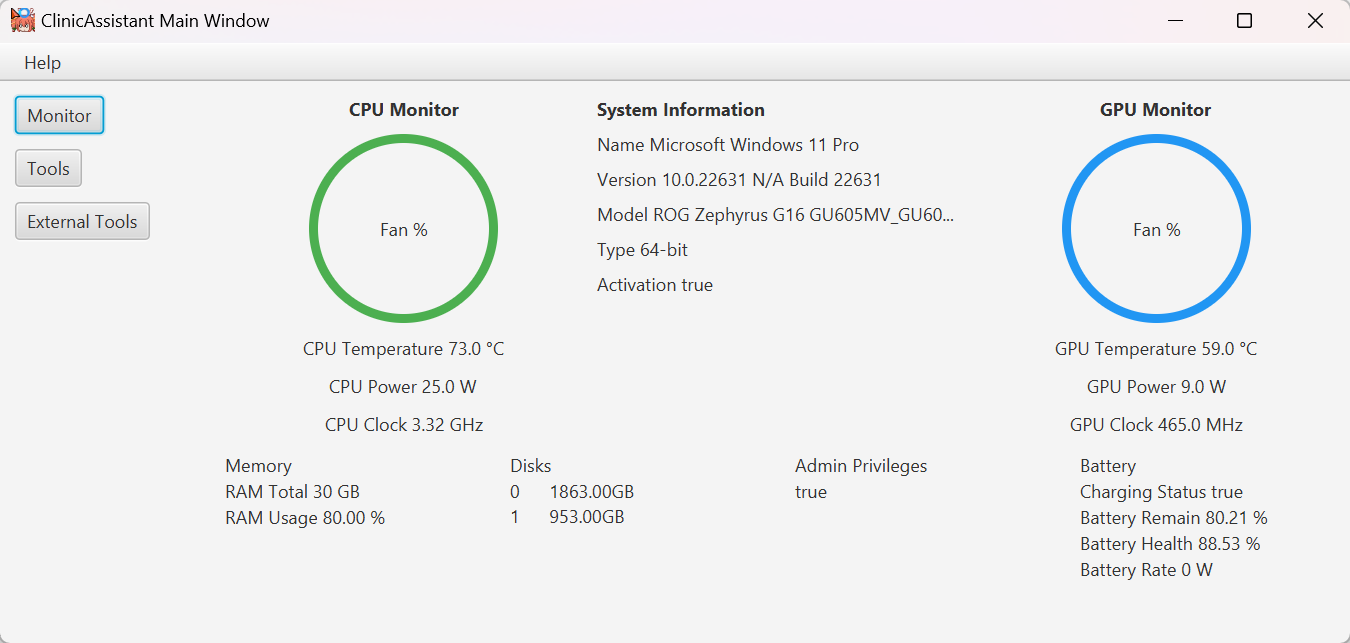
\includegraphics[
    width=0.95\linewidth,
    height=0.56\textheight,
    keepaspectratio
  ]{assets/clinic-assistant-monitor.png}
  \note{那第一学期做什么项目呢？大家以后一定会听说一位叫金旭亮的老师，他非常厉害。他大二上有一门计算机学院的专业限选课，就是java开发，我当时是诊所的部长，做了一个软硬件信息检测和调用维修工具的程序，叫clinic assistant。它算是我第一个认真写的项目，代码比较简单，大家可以可视化看到程序的样子，所以我们第一学期围绕它展开。
  为了说明我们要对这个项目具体做什么，我先介绍一个它实际工作的工作原理，就是它是如何获取硬件信息，比如CPU的温度信息的}
\end{frame}

\begin{frame}[fragile]{最开始收到的是指标和对应索引的映射}
  ClinicAssistant 借助 LibreHardwareMonitor 读取硬件信息。
  \par\medskip
  第一次先取得一段 \textbf{JSON 文本}，按固定格式列出能读取的指标。
  \par\bigskip
  \begin{columns}[T,onlytextwidth]
    \begin{column}{0.58\textwidth}
      \begin{lstlisting}[language={}]
[
  {"Name": "CPU Package",
   "Info": "Temperature", "Index": 7},
  {"Name": "CPU Package",
   "Info": "Power", "Index": 8},
  {"Name": "Memory Used",
   "Info": "Data", "Index": 20}
]
      \end{lstlisting}
    \end{column}
    \begin{column}{0.38\textwidth}
      \begin{itemize}
        \item \texttt{Name}：名称
        \item \texttt{Info}：指标类型
        \item \texttt{Index}：索引（编号）
      \end{itemize}
      \medskip
      列表告诉程序\alert{能读什么、用哪个编号读取}。
    \end{column}
  \end{columns}
  \par\medskip
  \note{首先，clinic assistant自己没有能力去读cpu温度这种信息，它是借助了一个叫libre hardware monitor的东西读的，简称LHM。首先它先问这个LHM获取它能读到的信息的列表，也就是左边这样。每个指标有它的名字，指标类型和索引编号。}
\end{frame}

% \begin{frame}{程序把文本拆成一条条记录}
%   按 JSON 的格式识别名称、类型和编号，这一步叫\textbf{解析}。
%   \par\bigskip
%   \centering
%   \begingroup
%   \renewcommand{\arraystretch}{1.6}
%   \begin{tabular}{lll}
%     \textbf{名称（Name）} & \textbf{类型（Info）} & \textbf{编号（Index）} \\
%     \hline
%     \texttt{CPU Package} & \texttt{Temperature}（温度） & 7 \\
%     \texttt{CPU Package} & \texttt{Power}（功率） & 8 \\
%     \texttt{Memory Used} & \texttt{Data}（数据量） & 20 \\
%   \end{tabular}
%   \endgroup
%   \par\bigskip
%   \begin{itemize}
%     \item 原来是一整段文字，现在可以逐条取出里面的信息。
%   \end{itemize}
% \end{frame}

\begin{frame}{根据索引读取对应的数值}
  清单告诉我们指标的名称和索引；要取得\textbf{当前数值}，还需要按索引请求读取。
  \par\bigskip
  \begin{enumerate}
    \item \textbf{查到 CPU 温度对应的索引是 7}\par
      清单中，\texttt{CPU Package} 的 \texttt{Temperature} 对应 \texttt{Index: 7}。
    \item \textbf{把索引 7 发给 LHM 辅助程序}\par
      ClinicAssistant 请求：“请读取索引 7 对应的当前数值。”
    \item \textbf{收到返回值 50}\par
      请求的是 CPU 温度，因此这次读到的温度是 \alert{50\,°C}。
  \end{enumerate}
  \note{刚刚那些相当于只是这些指标的名字，我们要想获得具体的值，就得把指标对应的索引发给LHM。比如我们要读第一个CPU温度，那就告诉LHM，我们要索引7的值，它就会把值给我们了。}
\end{frame}

\begin{frame}{用编号读取数值，再保存到程序里}
  ClinicAssistant更新读数，再按记住的编号取值。
  \par\bigskip
  \centering
  \begin{tikzpicture}[
    node distance=7mm,
    stage/.style={
      draw=TalkAccent, rounded corners, align=center,
      inner sep=6pt, text width=0.25\textwidth,
      minimum height=18mm
    },
    ar/.style={-{Latex[length=2mm]}, thick, draw=TalkAccent}
  ]
    \node[stage] (request) {请求编号 \textbf{7}\\对应的读数};
    \node[stage, right=of request] (receive) {收到数值\\\textbf{50}};
    \node[stage, right=of receive] (save) {保存到程序里\\CPU 温度：\textbf{50}};
    \draw[ar] (request) -- (receive);
    \draw[ar] (receive) -- (save);
  \end{tikzpicture}
  \par\bigskip
  \begin{itemize}
    \item 程序知道自己问的是 CPU 温度，就把 50 存到对应位置。
    \item 下次读到 51，就把保存的温度更新成 51。
  \end{itemize}
  \note{之后程序可以把这个数值存起来，供图形界面去调用}
\end{frame}

% \begin{frame}{硬件信息怎样显示到界面上}
%   以显示 CPU 温度为例，看看一个读数经过哪些地方。
%   \par\bigskip
%   \centering
%   \begin{tikzpicture}[
%     node distance=6mm,
%     stage/.style={
%       draw=TalkAccent, rounded corners, align=center,
%       inner sep=6pt, text width=0.24\textwidth,
%       minimum height=16mm
%     },
%     ar/.style={-{Latex[length=2mm]}, thick, draw=TalkAccent}
%   ]
%     \node[stage, text width=0.32\textwidth] (read) {LibreHardwareMonitor\\读取温度};
%     \node[stage, right=of read] (data) {ClinicAssistant\\接收并保存读数};
%     \node[stage, right=of data] (ui) {UI（用户界面）\\显示温度和单位};
%     \draw[ar] (read) -- (data);
%     \draw[ar] (data) -- (ui);
%   \end{tikzpicture}
%   \par\bigskip
%   \begin{itemize}
%     \item UI 取出保存的温度 50，加上名称和单位，显示“CPU 温度：50\,°C”。
%     \item 程序反复读取，界面定时刷新，让我们看到温度变化。
%   \end{itemize}
% \end{frame}

\begin{frame}{同一个流程，可以有不同的实现}
  刚才展示了一种做法。仅仅是\textbf{什么时候查找索引}，就有多种选择。
  \par\bigskip
  \begin{enumerate}
    \item \textbf{每次读取前都查找}\par
      每次获取 CPU 温度，都先从清单中找到编号，再读取数值。
    \item \textbf{第一次用到时查找并保存}\par
      后续直接使用已存的编号；需要判断这个指标是否已经查过。
    \item \textbf{程序启动时集中查找}\par
      先找齐所有需要的编号，后续直接使用；启动时要做更多准备。
  \end{enumerate}
  \bigskip
  \alert{重复查找的开销、准备工作的时机、代码的复杂程度，都需要权衡。}
  \note{说这个例子是想说明一个事情，就是像刚刚这样一个流程，中间的步骤都有很多不同的实现方法。比如（读）}
\end{frame}

\section{第一学期的计划}

\begin{frame}{第一学期：在小任务中练习设计}
  第一学期主要就是围绕这样的流程，练习设计、实现和改进。
  \par\bigskip
  \begin{itemize}
    \item \textbf{重写一个已有功能}\par
      每次选取流程中的一小部分，小组讨论如何设计、如何实现。
    \item \textbf{阅读并理解已有代码}\par
      理解代码如何组织、如何设计、如何实现，
      也可以试着找找原有的 bug 和不足。
    \item \textbf{整个过程都在小组内分工进行}\par
      从阅读代码、讨论设计，到编写、检查和整合，都由组员分工协作。
  \end{itemize}
  \note{所以呢，我们今年就是围绕一些这样的流程，比如给出某一部分功能的详细描述，大家组内去讨论研究怎么写，然后分工写代码。或者就是让大家去阅读一些已有的代码，理解（读）。当然，整个过程都在小组分工内进行，（读）}
\end{frame}

\begin{frame}{第一学期怎么安排}
  \begin{enumerate}
    \item \textbf{前两次分享会：认识基本概念，做简单练习}\par
      安装开发工具，熟悉基本操作。
    \item \textbf{第二次分享会后：分组，开始项目}\par
      每组五人，由一位部长指导；结合空闲时间和组队意愿安排。
    \item \textbf{后两次分享会及之后：边学边做}\par
      把 ClinicAssistant 的功能拆成小任务，逐步重新实现。\par
      每周统一给出任务，组会上回顾进展、讨论问题。
  \end{enumerate}
  \bigskip
  \alert{组会每周不超过 1 小时，独立写代码每周不超过 3 小时。}
  \note{不过也不是我们一开始就要组队的，毕竟最开始你还啥都不会嘛。所以呢，我们最开始两次技术分享会后才开始组队，这两次（读）}
\end{frame}

\section{怎么继续学}

\begin{frame}{分享会之外，怎么学}
  \begin{columns}[T,onlytextwidth]
    \begin{column}{0.47\textwidth}
      \textbf{分享会：建立整体认识}
      \medskip
      \begin{itemize}
        \item 有哪些知识，它们怎样关联。
        \item 一个工具为什么存在，能解决什么问题。
      \end{itemize}
    \end{column}
    \begin{column}{0.47\textwidth}
      \textbf{课后自学与实践：掌握具体内容}
      \medskip
      \begin{itemize}
        \item 根据学习资料，自主学习具体知识和用法。
        \item 通过练习和小任务，把学到的内容用起来。
      \end{itemize}
    \end{column}
  \end{columns}
  \bigskip
  \bigskip
  我们会提供入门资料，由部长指导小组实践。
  \par\medskip
  \alert{遇到问题，可以在群里提问，也可以带到组会上一起讨论。}
  \note{不过呢，由于分享会时间有限，我们只能概述性地讲讲，让大家对知识留个印象（读）。之后还是需要大家下去自己学具体的内容，我们也会有一些帮助大家巩固知识的小练习之类。不会很多，毕竟我们就是为了学习软件开发的。（读）}
\end{frame}

\end{document}
